\chapter{Tracking And Processing The Line Using Image Processing}
\label{chap:camera}

In this section the methods for capturing images and performing the necessary processing are explained in detail, with emphasis on how the image is processed to produce an error signal for the control system.

%
%
%
%
\section{Capturing The Image}
As explained in the introduction, the camera used for this project is a Sony PS3 Eye camera, which is based on OmniVision's OV543 camera sensor. All image capture and processing is carried out in the Raspberry Pi running the Raspbian Linux distribution.

The PS3 Eye camera is supported directly by the Linux kernel, and can be controlled by user software through the Video4Linux driver interface. The PS3 Eye camera was chosen for this project, because of its specification and low price. The camera is capable of shooting 125 frame per second, why it is perfect for computer vision applications (what is actually also was made for).

When the robot starts, the camera is set up to deliver 30 frames per second, in gray-scale colors. As part of the initialization, a callback is given to the camera module, and is called every time a new frame is ready for processing. We will not go further into the specific code, but just notice that it may be found in the `camera.h` and `camera.c` source files (see appendix). 

Figure \ref{fig:camera_1} shows two raw images of the line, captured by the camera. Later in this chapter, we will shows how the image extracts the line, and calculates the error signal.

\begin{figure}[!ht]
	\centering
	\subfloat[Straight line]{%
		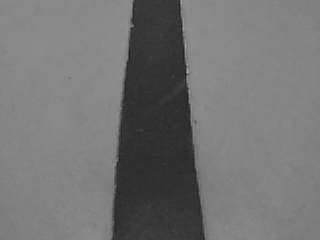
\includegraphics[width=0.4\textwidth]{resources/img-straight}
		\label{fig:camera_1_1}}
	\subfloat[Intersection]{%
		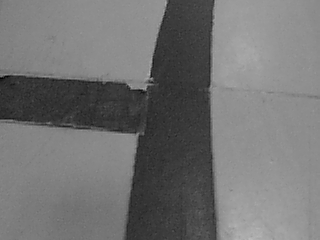
\includegraphics[width=0.4\textwidth]{resources/img-intersection}
		\label{fig:camera_1_2}}
	\caption{Raw images captured by the camera}
	\label{fig:camera_1}
\end{figure}


%FPS, size, camera angle, camera height.
%Playstation3 Eye Camera, OV534 sensor, Video4Linux driver, memory mapped files for faster access.
%Limitations of the frame rate.

%
%
%
%
\section{Identifying and Extracting the Line}

Whenever an image has been captured and is available in the memory, it is time to do the image processing and extract the line from the background. This is done using the steps listen below.

\begin{itemize}
	\item Contrast and brightness is adjusted
	\item The image is `sliced` into six horizontal slices
	\item For each slice, a histogram is calculated, and from that a optimum thresholding value
	\item Finally each pixel in each slice is marked as LINE if below the threshold value, or marked as FLOOR if above the threshold value
\end{itemize}

%
%
%
%
\subsection{Contrast and brightness}

In the following sections when referring to the image data, a simple notation will be used. The input image is given as $f(x,y)$, and the output image is given as $g(x,y)$, where $x$ and $y$ are the coordinates of a given pixel. 

The contrast and brightness adjustments are simple point-processing operations, which can be describes with the following equation.
\begin{equation}
	g(x,y) = a \cdot f(x,y) + b
\end{equation}

The brightness $b$ changes the overall brightness of the image, thus making all individual pixel more brighter. The contrast adjusted by $a$ simply makes the contrast between the individual pixels bigger.

In the system the possibility of changing the brightness and contrast are available, but at time of writing, the configuration is set to $a = 1$ and $b = 0$, i.e. no changes in brightness or contrast.


%
%
%
%
\subsection{Slicing}

Due to huge changes in the illumination of the image, it is split into five horizontal slices. For each of these slices a histogram is calculated, and a thresholding value is found. By doing this instead of one thresholding value for the whole image, we obtain a much better thresholding. 

\begin{figure}[!ht]
	\centering
	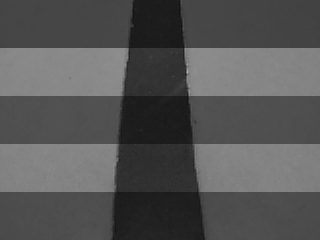
\includegraphics[width=0.4\textwidth]{resources/img-line-straight-raw-sliced}
	\caption{Raw image with slices marked}
	\label{fig:camera_2}
\end{figure}


%
%
%
%
\subsection{Histogram}

Whenever the images are sliced into slices, a histogram for each slice is calculated. A histogram shows the distribution of pixels of different color values. The typical histogram of a gray-scale image shows the color values on the x-axis $[0-255]$, and the percentage of the given color on the y-axis $[0-1]$. The value 0 on the x-axis is the black colors, whereas the value 255 is the white colors. With this in mind, we can conclude that the first hill on the histogram is the line, centered around 50, and the second hill is the floor, centered around 135.

\begin{figure}[!ht]
	\centering
	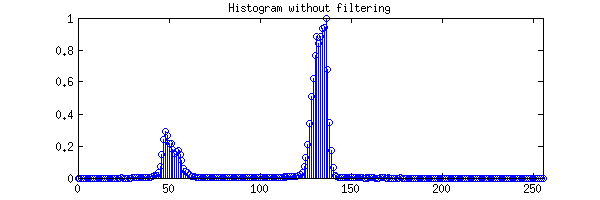
\includegraphics[width=0.8\textwidth]{resources/hist-no-filter}
	\caption{Histogram without filtered}
	\label{fig:camera_3}
\end{figure}

Figure \ref{fig:camera_3} shows the histogram of a slice from the image in figure \ref{fig:camera_2}. A lot of noise is visible on the histogram, which makes calculating the correct thresholding point less accurate. Hence, the histogram is filtered by a 16-point/length moving average filter, which gives the histogram shown in figure \ref{fig:camera_4}.

\begin{figure}[!ht]
	\centering
	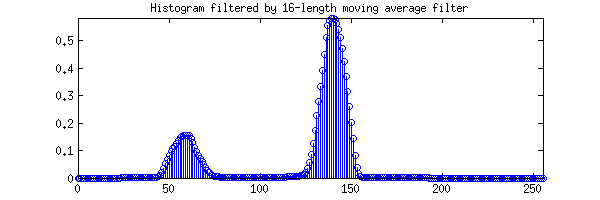
\includegraphics[width=0.8\textwidth]{resources/hist-filter}
	\caption{Histogram filtered with 16-point average filter}
	\label{fig:camera_4}
\end{figure}

The filtered histogram has less spikes, and is much better when applying the Optimum Thresholding algorithm in the next section.


%Figure: Image before thresholding, histogram of the same image (use MATLAB's imhist and imread)

%
%
%
%
\subsection{Optimum thresholding}

Next, when the pretty averaged histogram is calculated, it is time to calculate the perfect threshold value for segmenting the line from the floor - in other words, finding the value on the x-axis of the histogram where a clear split between the colors of line and colors of the floor is to be found.

The Optimum Thresholding algorithm is described in \citep{myler1993}, which also provides a reference implementation in C. This implementation is fitted into our existing code base, and used without major modifications.  

The algorithms work by iterating through the histogram, finding the first valley. That is, by looking at a single color on the x-axis, where the color to the left has a larger or equal percentage, than the current color, and color to the right has a small percentage. If $h[x]$ is the histogram, then equation \ref{eq:camera_1} describes the valley.

\begin{equation}\label{eq:camera_1}
	h[x-1] \geq h[x] < h[x+1]
\end{equation}

Figure \ref{fig:camera_5} shows the histogram zoomed in around the first valley after the top of the first hill (the line). Equation \ref{eq:camera_1} is satisfied first time at about $x = 115$, which in this case will be the optimum thresholding value.

Listing \ref{lst:camera_1} shows part of the implementation of optimum thresholding from image.c. In the while-loop from line 1-9, the histogram is iterated through, and a flag is set when equation \ref{eq:camera_1} is fulfilled.

\begin{figure}[!ht]
	\centering
	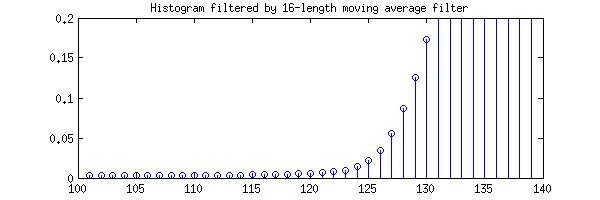
\includegraphics[width=0.8\textwidth]{resources/hist-zoom-valley}
	\caption{Histogram zoomed in before the `floor` hill}
	\label{fig:camera_5}
\end{figure}


\lstset{language=C,basicstyle=\tiny,numbers=left}
\begin{figure}
\begin{lstlisting}[frame=single,caption=Part of the thresholding code,label=lst:camera_1]
	while (flag == 0 && y < 254)
	{
		if (hist[y-1] >= hist[y] && hist[y] < hist[y+1]) 
		{
			flag = 1;
			thr = y;
		}
		y++;
	}
	for (j = start; j < end; j++)
	{
		buffer[j] = buffer[j] < thr ? LINE : FLOOR;
	}
\end{lstlisting}
\end{figure}

Finally, when the threshold value is calculated a slice, the image data is segmented using that value. The mathematical description of thresholding is given en equation \ref{eq:camera_2}.

\begin{equation}\label{eq:camera_2}
\begin{split}
	\text{if } f(x,y) \leq T \text{ then } g(x,y) = 0 \text{ (line) } \\
	\text{if } f(x,y) > T \text{ then } g(x,y) = 255 \text{ (floor)}
\end{split}
\end{equation}



Line 10-13 of listing \ref{lst:camera_1} loops through all pixels, and decides if they are line or floor. The images presented first in this chapter, is shown below in figure \ref{fig:camera_6} in their processed and segmented versions (all images are actual extract from the robots image processing system).

As we can see on figure \ref{fig:camera_6_2}, it has not been possible to find a optimal thresholding value, probably due to a too low contrast caused by sun light. In the right side of the image, only the edge of the line is marked as line. 

\begin{figure}[!ht]
	\centering
	\subfloat[Straight line]{%
		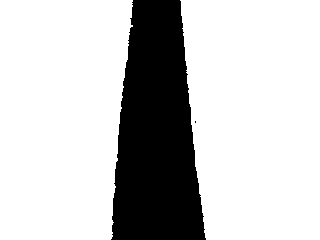
\includegraphics[width=0.3\textwidth]{resources/img-straight-thr}
		\label{fig:camera_6_1}}
	\subfloat[Intersection]{%
		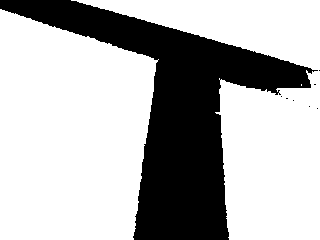
\includegraphics[width=0.3\textwidth]{resources/img-intersection-thr}
		\label{fig:camera_6_2}}
	\caption{The images after being processed}
	\label{fig:camera_6}
\end{figure}


%Moving average filter (16-length)
%Figure: Thresholded image, histogram illustration

%
%
%
%
\section{Calculating the Error Signal}

Now that the line is segmented from the floor, next step is BLOB (Binary Large OBject) analysis. \citep{moeslund2009} presents a bunch of techniques for classification of BLOBs, i.e. distinguishing different BLOBs from each other. Each of the different characteristics a BLOB may be represented by, is denoted a feature. Common features are area, bounding box, compactness, circularity. Another one is called `Center of mass`, which is the physical location on an object, where you should place a finger in order to balance the object. In terms of image processing, it is the average x- and y-positions of the binary object (the line). It is defined as a point whose x-point is calculated by summing the x-coordinates of all pixels in the BLOB and dividing by the total number of pixels. Likewise for the y-value. The `center of mass` feature is used to calculate the error signal the system.

In mathematical terms, the center of mass $(x_c, y_c)$ is defined as given in equation \ref{eq:camera_3}.

%Center of middle mass, multiple points, mass
%Figure: Image with error points

\begin{equation}\label{eq:camera_3}
	x_c = \frac{1}{N} \sum_{i = 1}^{N}{x_i} \quad \quad y_c = \frac{1}{N} \sum_{i = 1}^{N}{y_i} 
\end{equation}

Using the equation for center of mass, two error points are calculated for each image. One for the upper part of the image, which gives an indication of the error in the `future`, and an error point in the lower part of the image, which gives the actual present error. Figure \ref{fig:camera_7} shows the two images annotated with error points. The green line indicates the optimal direction of motion.

\begin{figure}[!ht]
	\centering
	\subfloat[Straight line]{%
		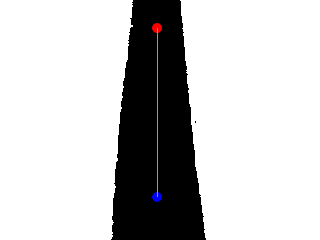
\includegraphics[width=0.4\textwidth]{resources/img-straight-thr-pt}
		\label{fig:camera_7_1}}
	\subfloat[Intersection]{%
		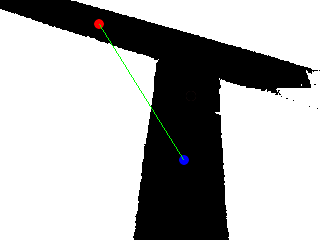
\includegraphics[width=0.4\textwidth]{resources/img-intersection-thr-pt}
		\label{fig:camera_7_2}}
	\caption{The images with two center of masses calculated}
	\label{fig:camera_7}
\end{figure}



%\section{Performance Considerations and Possible Improvements}
%Frame rate, further processing, light
